\begin{strip}
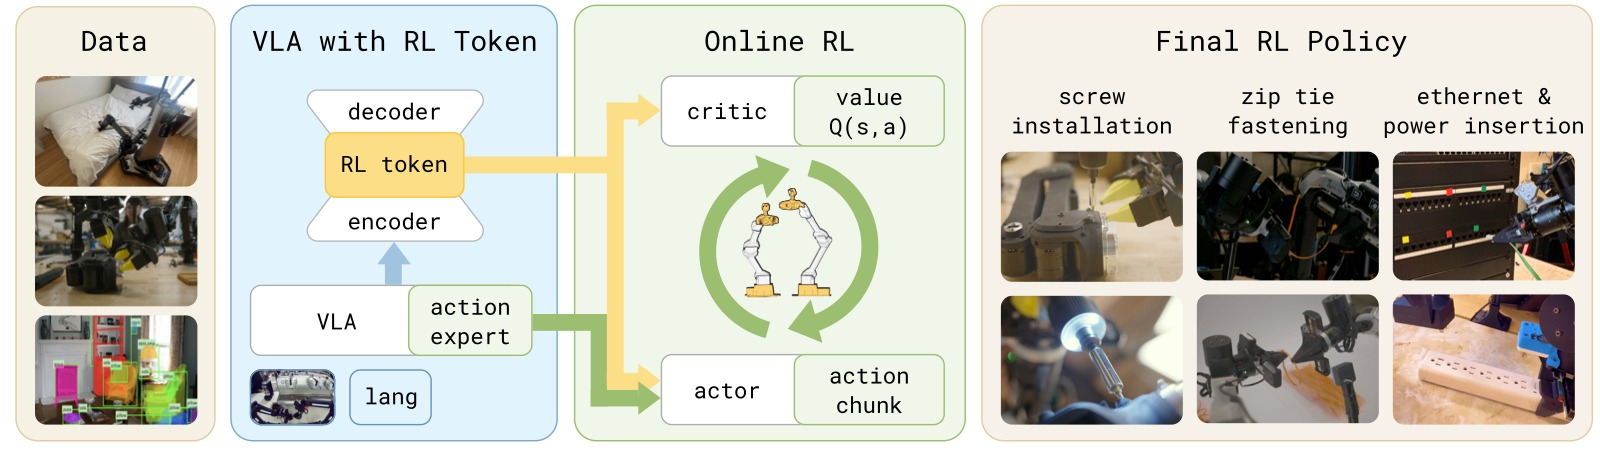
\includegraphics[width=\textwidth]{figs/overview.pdf}
%%SL.3.18: should we replace "readout token" with "RL token"? otherwise it's unclear why there is both a readout token and RL token; also make sure to use final names of each task (ziptie -> zip tie?)
    \captionof{figure}{Our method introduces an ``RL token'' into the VLA by training an encoder and decoder to produce a compact and meaningful representation from a VLA's internal features. The extracted representation is then used to train lightweight actor-critic networks with sample-efficient online RL, enabling very precise tasks to be fine-tuned with a few hours or even minutes of robot experience.}
    \label{fig:overview}
\end{strip}

\begin{abstract}
Vision-language-action (VLA) models can learn to perform diverse manipulation skills ``out of the box,'' but achieving the precision and speed that real-world tasks demand requires further fine-tuning -- for example, via reinforcement learning (RL).
We introduce a lightweight method that enables sample-efficient online RL fine-tuning of pretrained VLAs using just a few hours of real-world practice. We (1) adapt the VLA to expose an ``RL token,'' a compact readout representation that preserves task-relevant pretrained knowledge while serving as an efficient interface for online RL, and (2) train a small actor-critic head on this RL token to refine the actions, while anchoring the learned policy to the VLA. 
Online RL with the RL token (\MethodName{}) makes it possible to fine-tune even large VLAs with RL quickly and efficiently.
%Data produced by our RL method during deployment can be distilled back into the base VLA, resulting in a data flywheel that improves the foundation model itself through successive RL post-training cycles. 
Across four real-robot tasks (screw installation, zip tie fastening, charger insertion, and Ethernet insertion) \MethodName{} improves the speed on the hardest part of the task by up to 3$\times$ and raises success rates significantly within minutes to a few hours of practice. It can even surpass the speed of human teleoperation on some of the tasks. 
\end{abstract}